\documentclass[12pt,conference,onecolumn,titlepage]{IEEEtran} %This uses the IEEE template

%Set up for inputing Figures
\usepackage[pdftex]{graphicx}
\usepackage{wrapfig}
\usepackage[utf8]{inputenc}
%Include math packages
\usepackage{algorithmic}
\usepackage{pdflscape}
\usepackage{amssymb}
\usepackage{amsmath}
\usepackage{latexsym}
%Added Recommended packages
\usepackage{csquotes}
\usepackage[backend=biber]{biblatex}
\usepackage{hyperref}
\usepackage{cleveref}

% Include packages for line spacing
\usepackage{setspace}
\usepackage{parskip}
\usepackage{indentfirst}
\usepackage{verbatim}
\usepackage{adjustbox}
\usepackage{listings}
% \usepackage{subfigure}          
\usepackage{subcaption}
\usepackage[T1]{fontenc}
\usepackage[scaled]{beramono}
\newcommand\Small{\fontsize{9}{9.2}\selectfont}
\newcommand*\LSTfont{\Small\ttfamily\SetTracking{encoding=*}{-60}\lsstyle}

\addbibresource{/home/ivan/Dropbox/Documents/Latex_Stuff/BibDB/AllEntries.bib}
%dont think I need to use the graphics path yet
\graphicspath{{/home/ivan/src/Internship_GTRI/Documentation/Images/}
{/home/ivan/src/Internship_GTRI/Documentation/Images/screenshot/}} %Change this to your path!!!

\DeclareGraphicsExtensions{.pdf,.jpeg,.jpg,.png} %Make sure your figure extension is included in this list

%simple command to add a figure 
%\myfigure{address}{caption}{width}{label}
\newcommand{\myfigure}[4]{
  \begin{figure}[h!]
      \centering
      \includegraphics[width=#3\textwidth]{#1}
      \caption{#2}
\label{#4}
    \end{figure}
}

%simple command to add a figure wrapped in text
%\myfigure{image/address}{R_L_PLACEMENT}{width_in_text_width}{caption}{label}
\newcommand{\mywrapfigure}[5]{
  \begin{wrapfigure}{#2}{#3\textwidth}
    \centering
    \includegraphics[width=#3\textwidth]{#1}
    \caption{#4}
\label{#5}
  \end{wrapfigure}
}

\newcommand*{\figuretitle}[1]{%
    {\centering%   <--------  will only affect the title because of the grouping (by the
    \textbf{#1}%              braces before \centering and behind \medskip). If you remove
    \par\medskip}%            these braces the whole body of a {figure} env will be centered.
}

%Set up spacing
\linespread{1.3} %This creates 1.5 spacing
\setlength{\parindent}{12pt} %Sets the length of the indent at the beginning of each paragraph.

%Start the document
\begin{document}

\title{Golem Wing: Resurrection}
\author{Students: Ivan Dario Jimenez\\
Alex Gurney \\
CS3651\\
Date Submitted: \today \\}

\maketitle

\section{Overview}
\label{sec:overview}
%General Stuff
The Golem Wing was originally invented by Saul Reynolds in collaboration with Mike Stilman. The idea was to have a balancing holonomic robot that would be able move in any orientation and direction in the plane as well as stay upright for future purposes of manipulation. After attempting to balance using an external computer for controls the project was abandoned and left to gather dust for years in the IRIM lab.\par
Today we present a revival of this project where we try to recreate and improve on their previous achievements with a modern embedded Linux system: the Raspberry Pi. On-boarding the computer paves the way for fully tether-free performance as well as a tighter control loop necessary for maintaining the robot balanced.\par
\section{Hardware}
\label{sec:hardware}
%General Introduction to all the physical stuff we had to do to get the GOLEM Wing back working
\subsection{Electrical}
\label{sec:electrical}
\begin{figure}
  \centering
  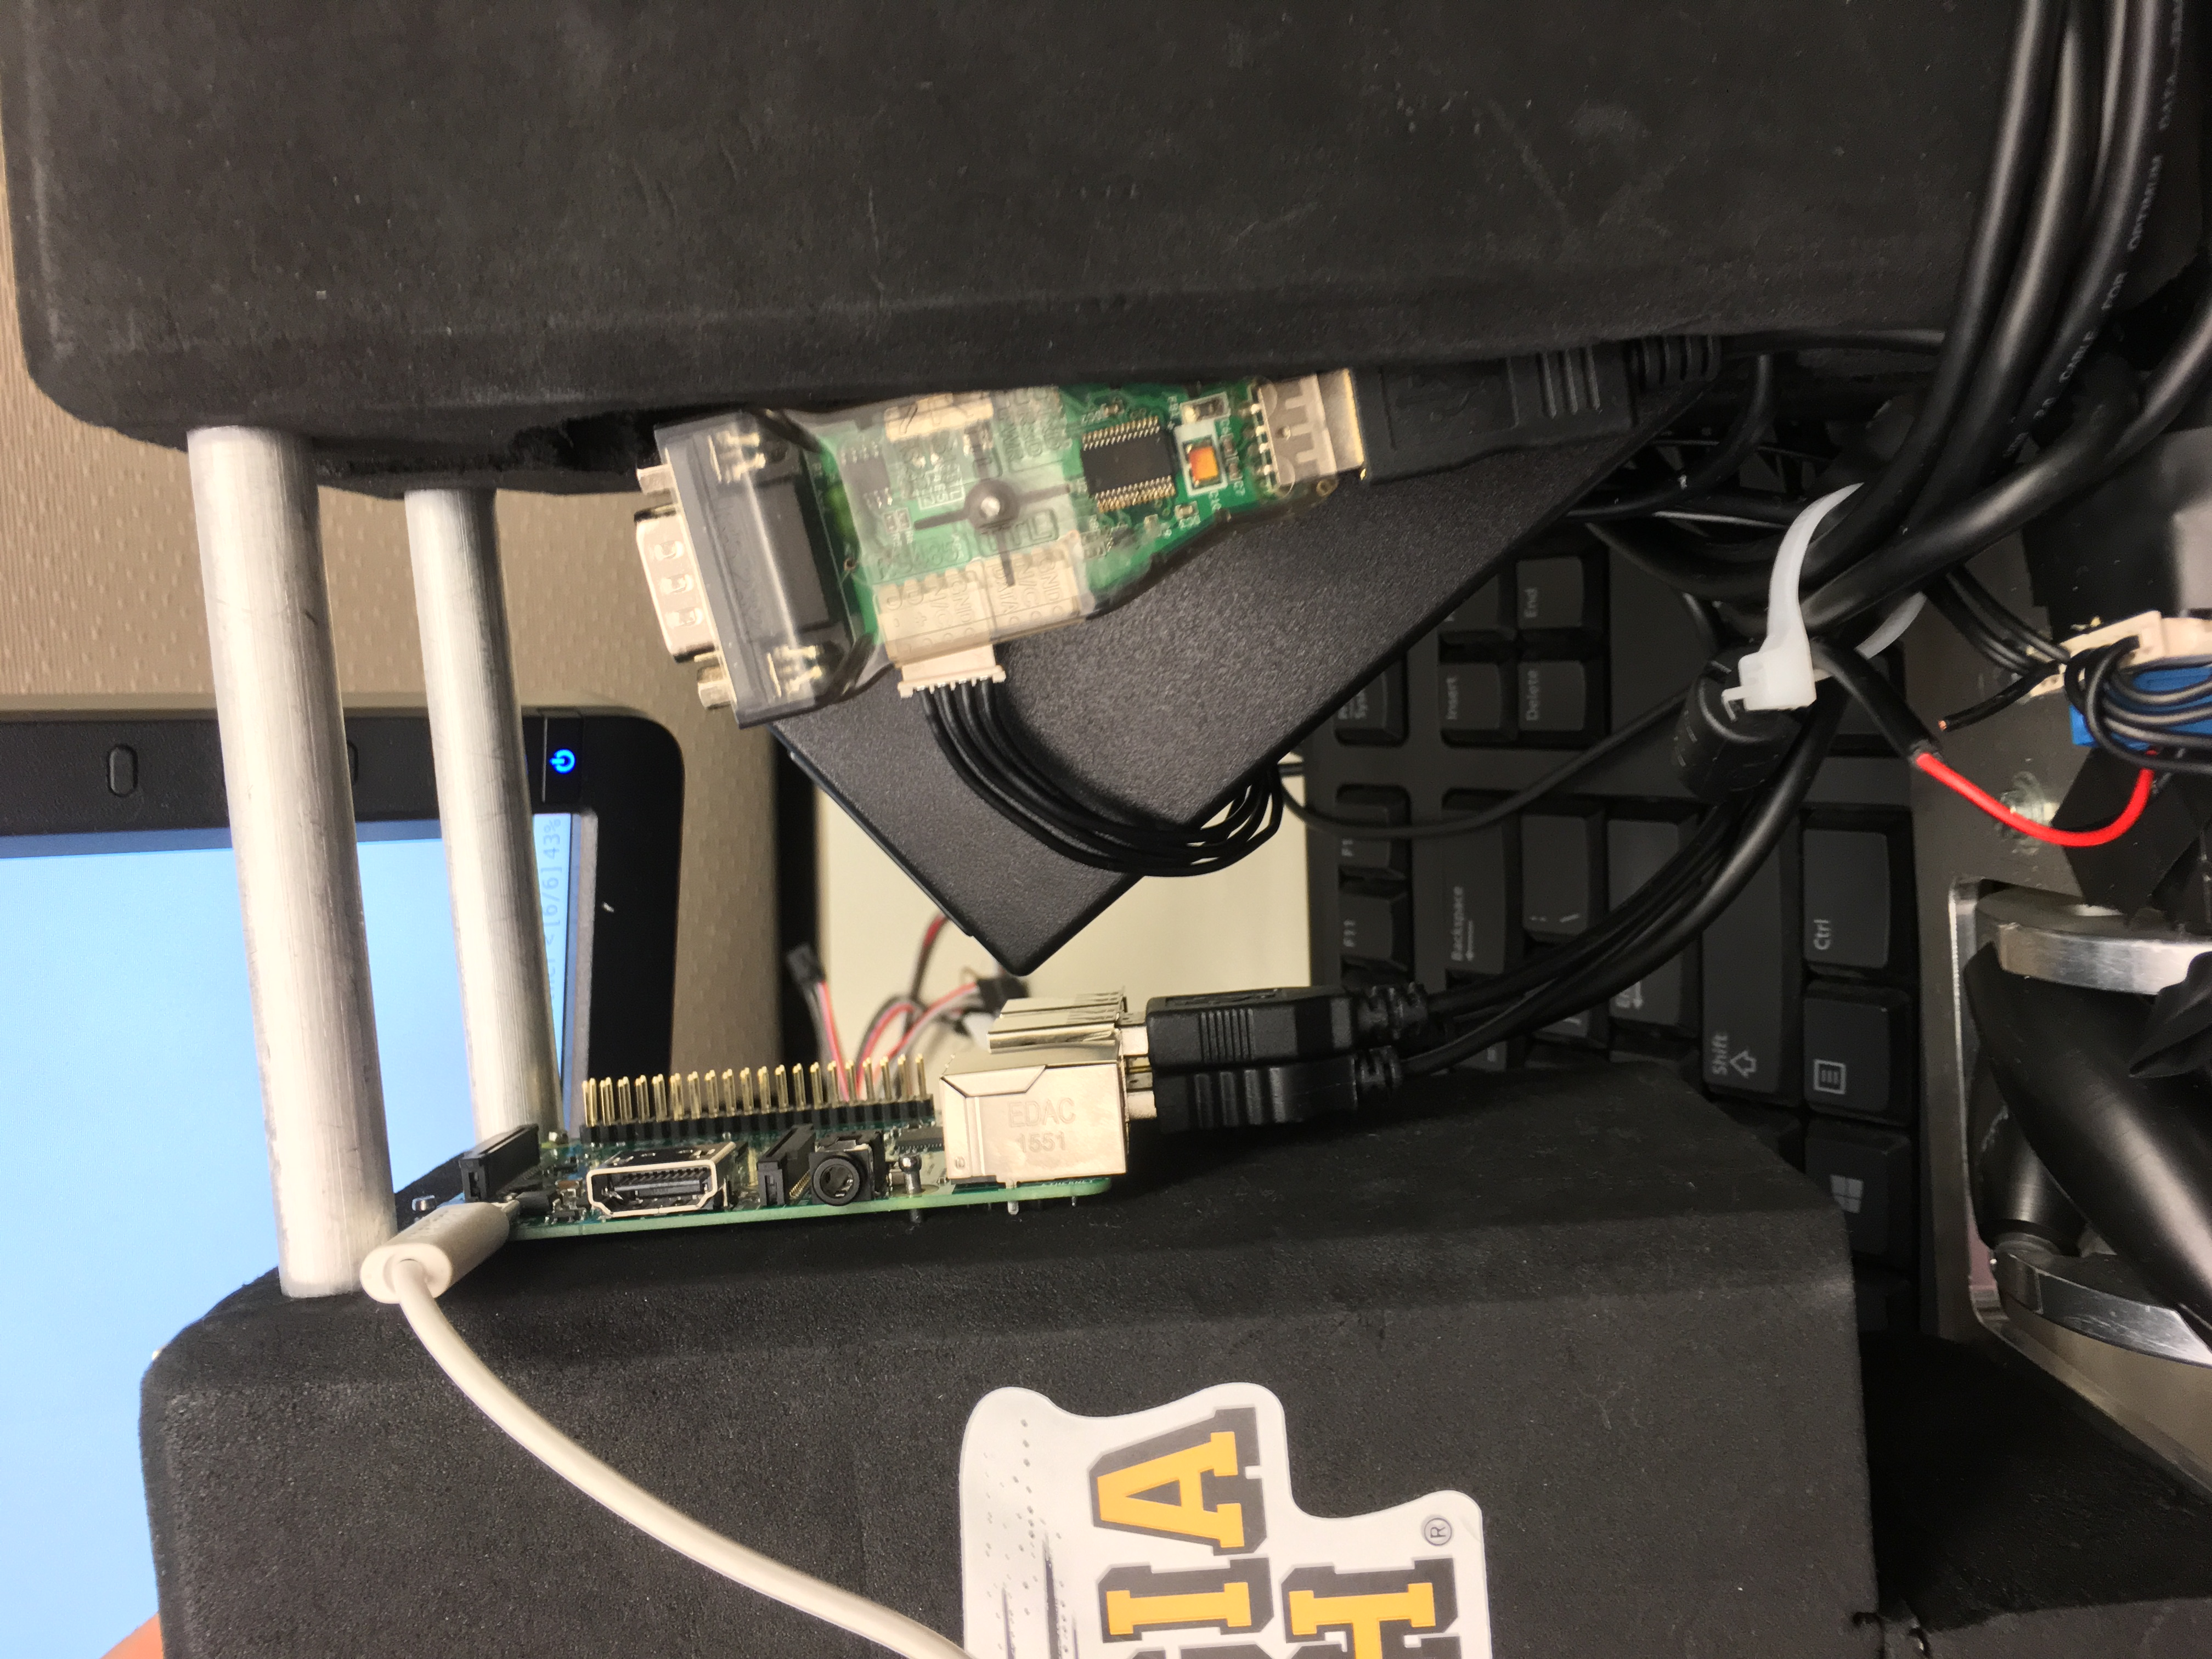
\includegraphics[width=1.0\textwidth]{cables.jpg}
  \caption{Internal electrical connections of the current iteration of the Golem Wing. You can see from left to right the Dynamixel Dongle, the Dynamixel DC power sourcde and the raspberry PI. On the bottom you can see the current connection between the dongle, the motors and the power souce. For illustrative purposes you can see the Dynamixel Dongle's VC cable cut.}
  \label{fig:cables}
\end{figure}
%The Iterations of connecting stuff. We should describe the iterative process of finding a better and better way to connect everything and make sure had a hardware stack comaptible with our software
Once our robot had mounted motors it needed an embedded micro-controller to drive them and to read sensor values. The final solution would have to aggregate a gyroscope, an accelerometer and a send commands to three motors in series.\par
The RX-24F motors connect with a 4 pin connector that has a ground, source and an RS485 bus. On top of the bus the motors require a custom proprietary package format in order to communicate with the motors.\par
Although the option of using the Teensy was thoroughly investiaged, the team opted for going with a different alternative. Using the Teensy would have required us to debug a packet protocol and a bus protocol at the same time without much feedback to determine what is wrong other than an oscilloscope. Although possible, it was outside the scope of time granted to complete the project. \par
Instead we opted for a Raspberry Pi which could run a ROS node that we knew could communicate with the motors. We tried using a Raspberry 2 but the required package was incompatible with the latest version of raspbian compatible with that machine. Since installation on the Raspberry Pi 2 was impossible we moved to a Raspberry Pi 3 which did support the required OS.\par
This was using a proprietary USB Dongle that translated form a USB serial connection to RS485. Since the Dongle and Raspberry cannot supply enough current to move all three motors we had to purchase a separate power supply. Our final solution involved connecting the power supply's ground and power to the ground and power of the motors, and the ground of the dongle. We passed through the Bus from the dongle to the motors and cut the source that came from the dongle from  the system. It was necessary to connect all grounds in order to ensure the that the BUS worked correctly.\par
With a suitable micro-controller we moved to connecting the desired sensor. We had to decide on the exact location since we had to choose between the top and bottom of the robot. We decided to to place the sensors as high on the robot as possible to increase sensitivity of the sensor. We worked at first with the ADXL345 accelerometer through the I2C bus.\par
Although The I2C bus was compatible with the Gyroscope 9-DoF stick solution we moved away from that because of a lack of libraries in the PI to read the values off the Gyroscope. This is because a Gyroscope needs to aggregate an accelerometer in order to avoid drift as well as translate the internal measurement to a meaningfull unit. Without a library to do those two things for us, completing the project in time would have been unrealistic. \par
Finally we opted for an Ardupilot that was pluggable into a USB port because there was a a library available that integrated well with our software stack.\par
\subsection{Mechanical} %alex
\label{sec:mechanical}

While many of the projects physical pieces were supplied by the sponsoring lab, a number of repairs and modifications were required. The robot initially only came with two motors, which were only partially mounted to the three supplied wheels. After researching supply options for a third motor, it was determined that mixing and matching motors and controller types was unfeasible. Luckily the sponsoring lab was able to supply another functional motor.

The motors' shafts were originally affixed to a proprietary attachment plate, which was bolted to a thick aluminum spacer, with pins extending from it, loosely fitting into radial slots to turn the wheel shaft. Unfortunately, there were only two of these plates, and the pins transferring power from the motors to the wheels created roughly 10 degrees of play in the system. The play was removed from the system, and the third wheel was attached by tightly bolting small spacers to the attachment plate. The bolt heads fit in the wheel's radial slots without play, and removed the requirement of the missing attachment plates.

While basic controls were being implemented, the Golem Wing was not yet able to balance. To allow for testing of the motors and control systems, a caster wheel was attached to the back of the robot, allowing it to remain upright naturally, even while in motion. To attach the caster wheel a plywood plank was cut on a bandsaw, holes were drilled, and it was mounted on top of the wing and cantilevered behind using zip ties. A cylindrical wooden rod was cut to the height of the robot and drilled into from one end. The caster wheel was screwed into this end, and the other end was cut at an angle and nailed to the plywood board to allow the caster to rotate freely about the vertical shaft while the robot leaned backwards, supported by it. Finally, when the control algorithms were complete, the caster wheel was removed, allowing the robot to intelligently balance unsupported.
\begin{figure}[h!]
  \centering
  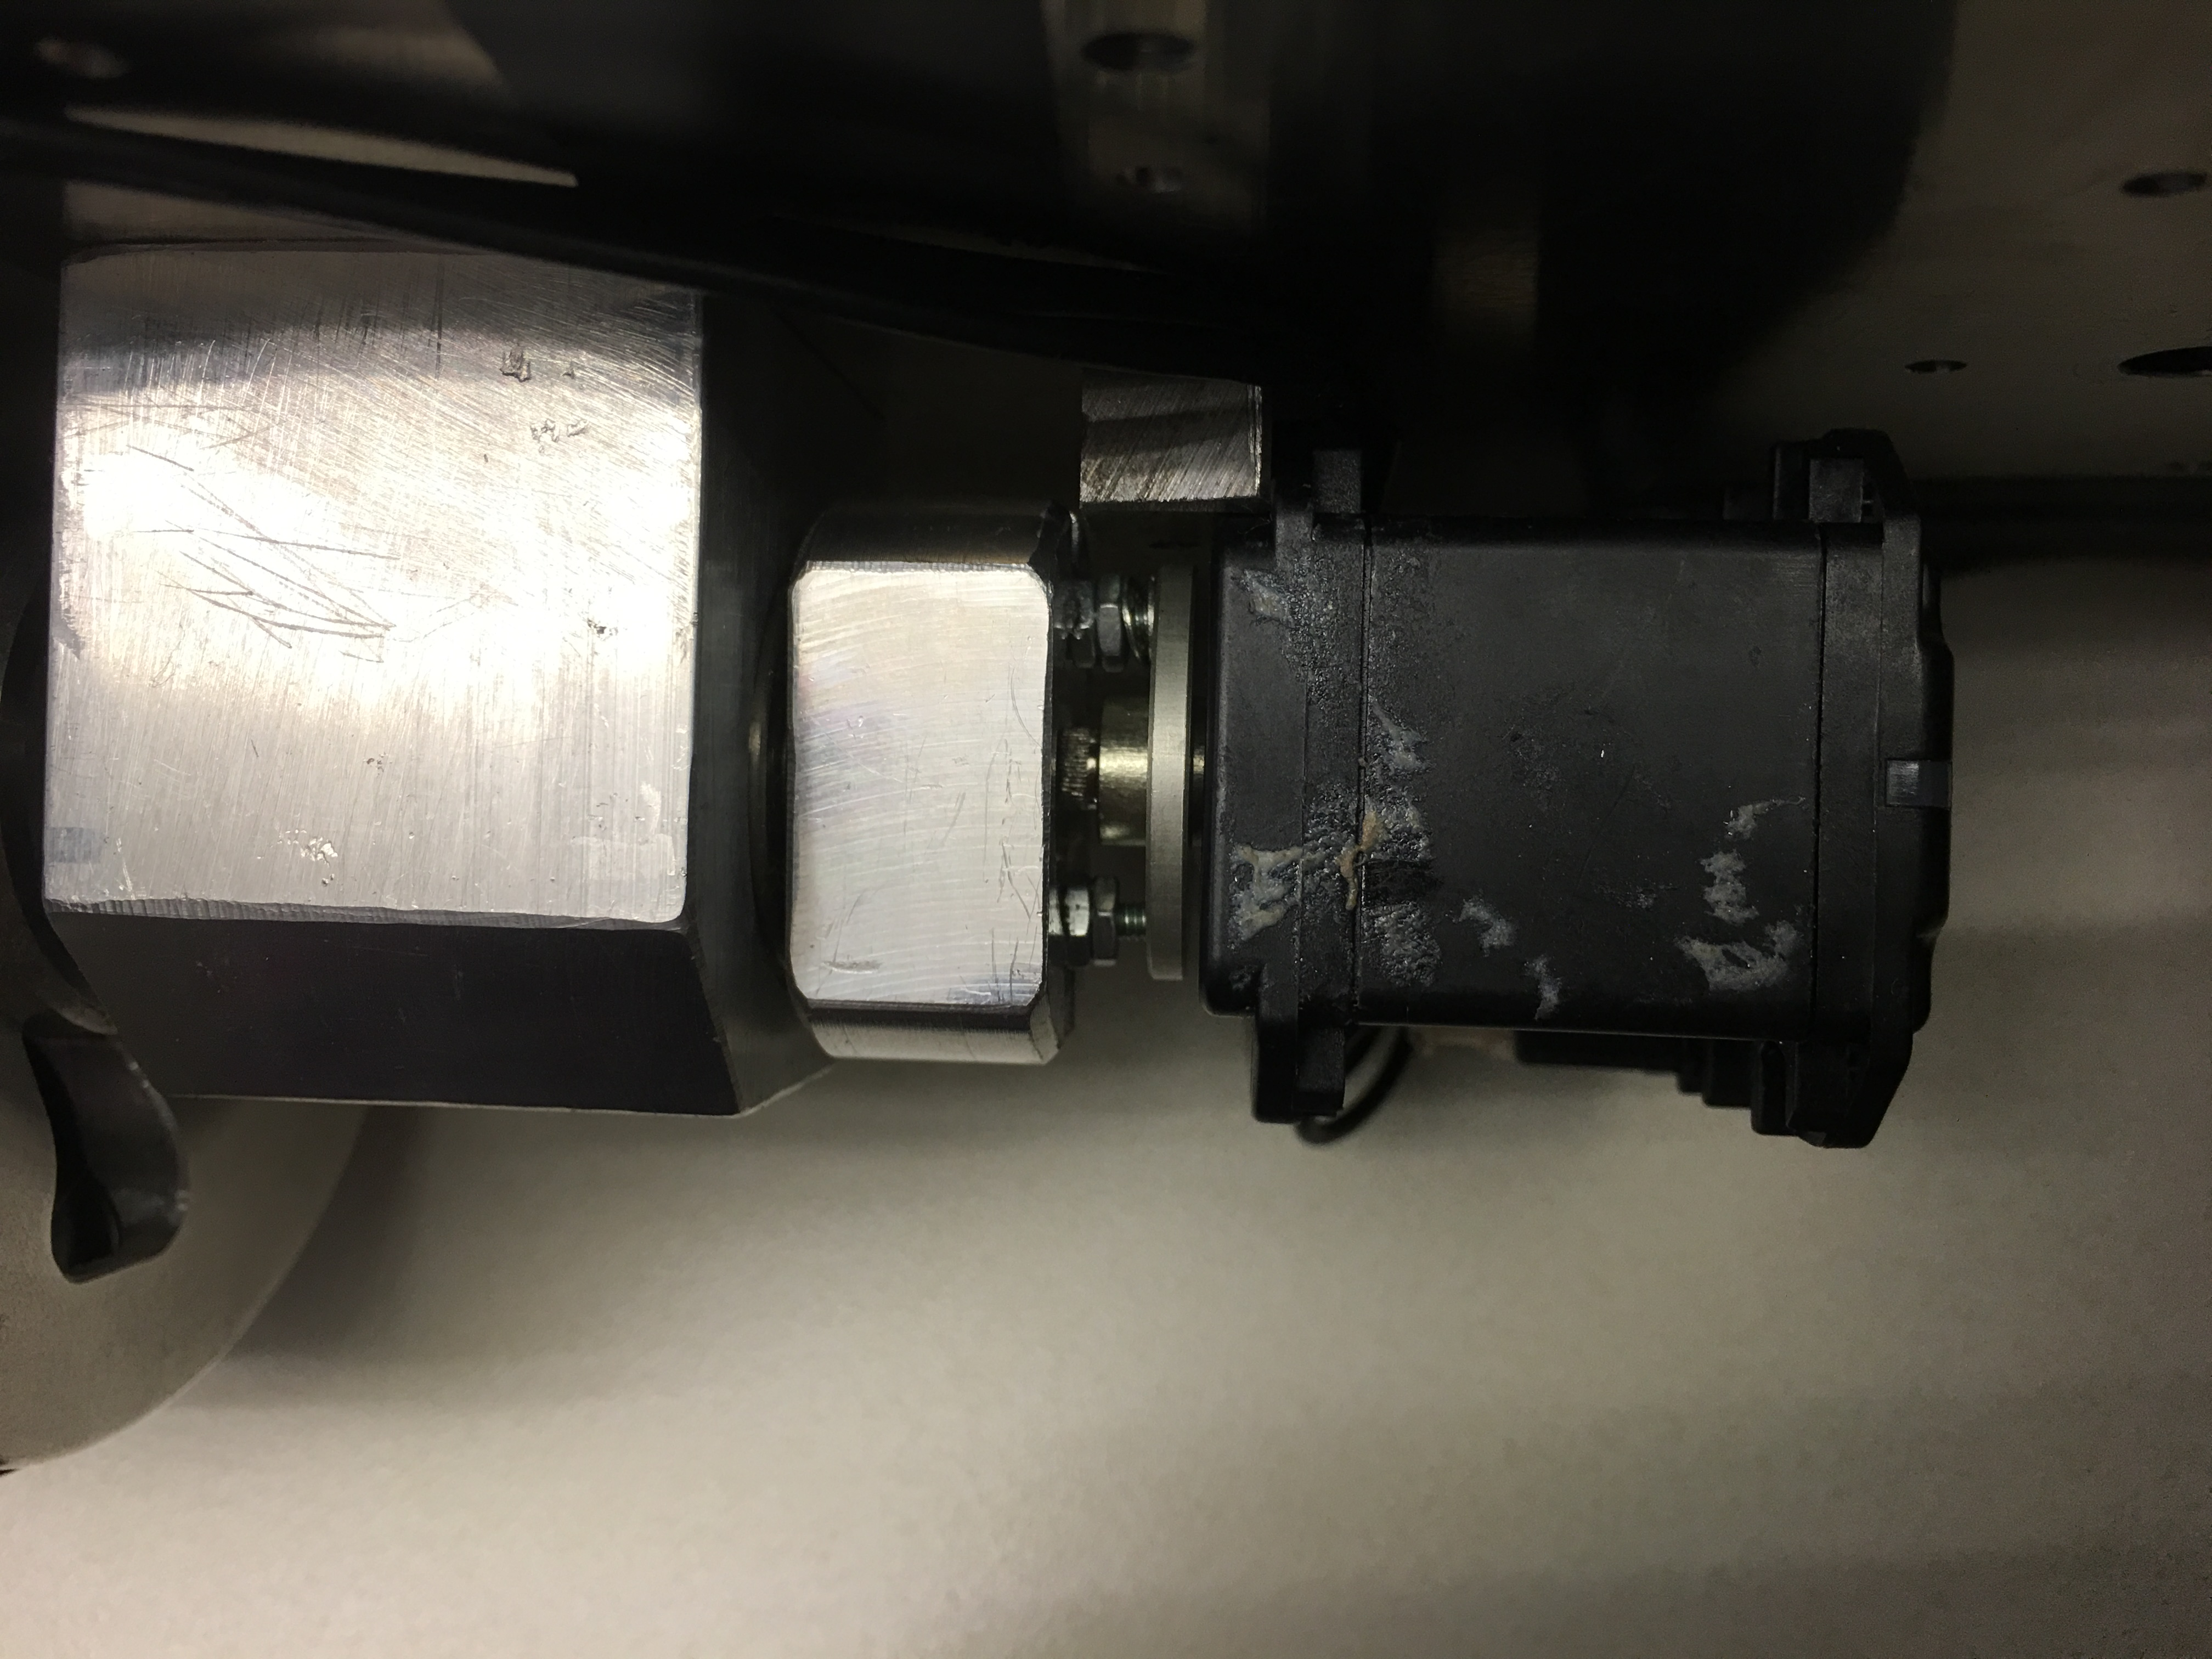
\includegraphics[width=\textwidth]{motor2bearing.jpg}
  \caption{Connection we built between the motor and the bearings.}
  \label{fig:motor2bearing}
\end{figure}

\section{Software}
\label{sec:software}
% 

\subsection{Previous Iterations}
\label{sec:previous-iterations}
% Talk about the previous ROS nodes for the accelerometer and any other thing we made but discarded

\subsection{ROS Application Architecture} % Alex
\label{sec:ros-appl-arch}
In order to efficiently interface with the numerous electronic devices tested and the ones eventually used in the final design, it was determined that the final project should be implemented in ROS (Robot Operating System). At its core, ROS has the goal of reducing the work required to implement robotics projects through code reuse and modularization, supported by a robust message passing system. For an overview of the architecture as implemented, please refer to the figure below.

\begin{figure}[h!]
  \centering
  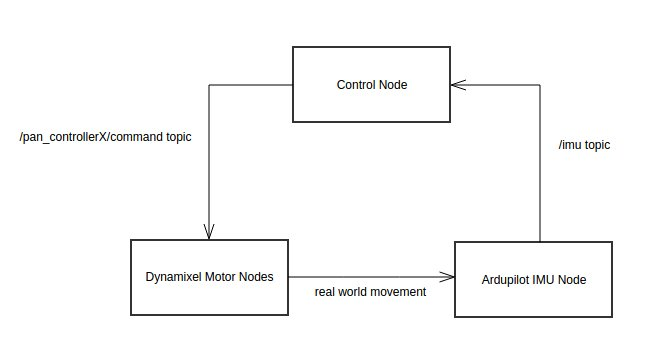
\includegraphics[width=\textwidth]{rosarcitecture.jpg}
  \caption{High Level Architecture of the ROS Project.}
  \label{fig:ROSArchitecture}
\end{figure}

Open source software was available for the Dynamixel motors, allowing us to simply install the Dynamixel ros node package, and start a Dynamixel node in our ros project for each of the three Dynamixel motors. The motors were controlled by issuing velocities through the ros topic system with our control node through the \text{$pan_controllerX command$} topic, where X is the motor ID.

An open source ros node was also available to manage communications with the ardupilot 9 DOF IMU. This node communicated with the Ardupilot IMU over a serial port, receiving serial data and constructing and publishing a ros $sensor_msgs/IMU message$. This message contains a lot of pose information, including orientations, which were used to inform the control node and maintain stability, as described in the Controls section below.

The control node was written entirely by us. It subscribed to the $/imu$ topic published by the ardupilot node, and published motor commands to the $/pan_controllerX/command$ topic. The control scheme will be detailed below, but the goal of this node is simply to send the motors commands to maintain balance.


\subsection{Controls} % Controls
\label{sec:controls}
The ROS node written for controlling the motion of the balance bot used a fairly simple PID control scheme. The PID control scheme records a single pitch orientation angle as the command angle, and then measures the current pitch angle and sends commands to motors in an attempt to achieve the commanded angle. The new signal at each time point is a combination of the P, I and D gains, and the current and previous errors observed.

For our robot, the best stability was found when P ~100 D~-1000 I~.09.

% Perhaps talk a b it about our investigation into the controller of the robot, specifically the iteresting soloutions we found for the IK that we implemented for our first presentation and then why we couldn't easily aggregate them into the final controller.


\section{Results}
\label{sec:results}
% A picture of the robot balancing. Maybe even a set of pictures showing how it balanced even though we kicked it. Explain why we got the results we got especially the instabilities and the reason it oscillated. 
\begin{figure}
  \centering
  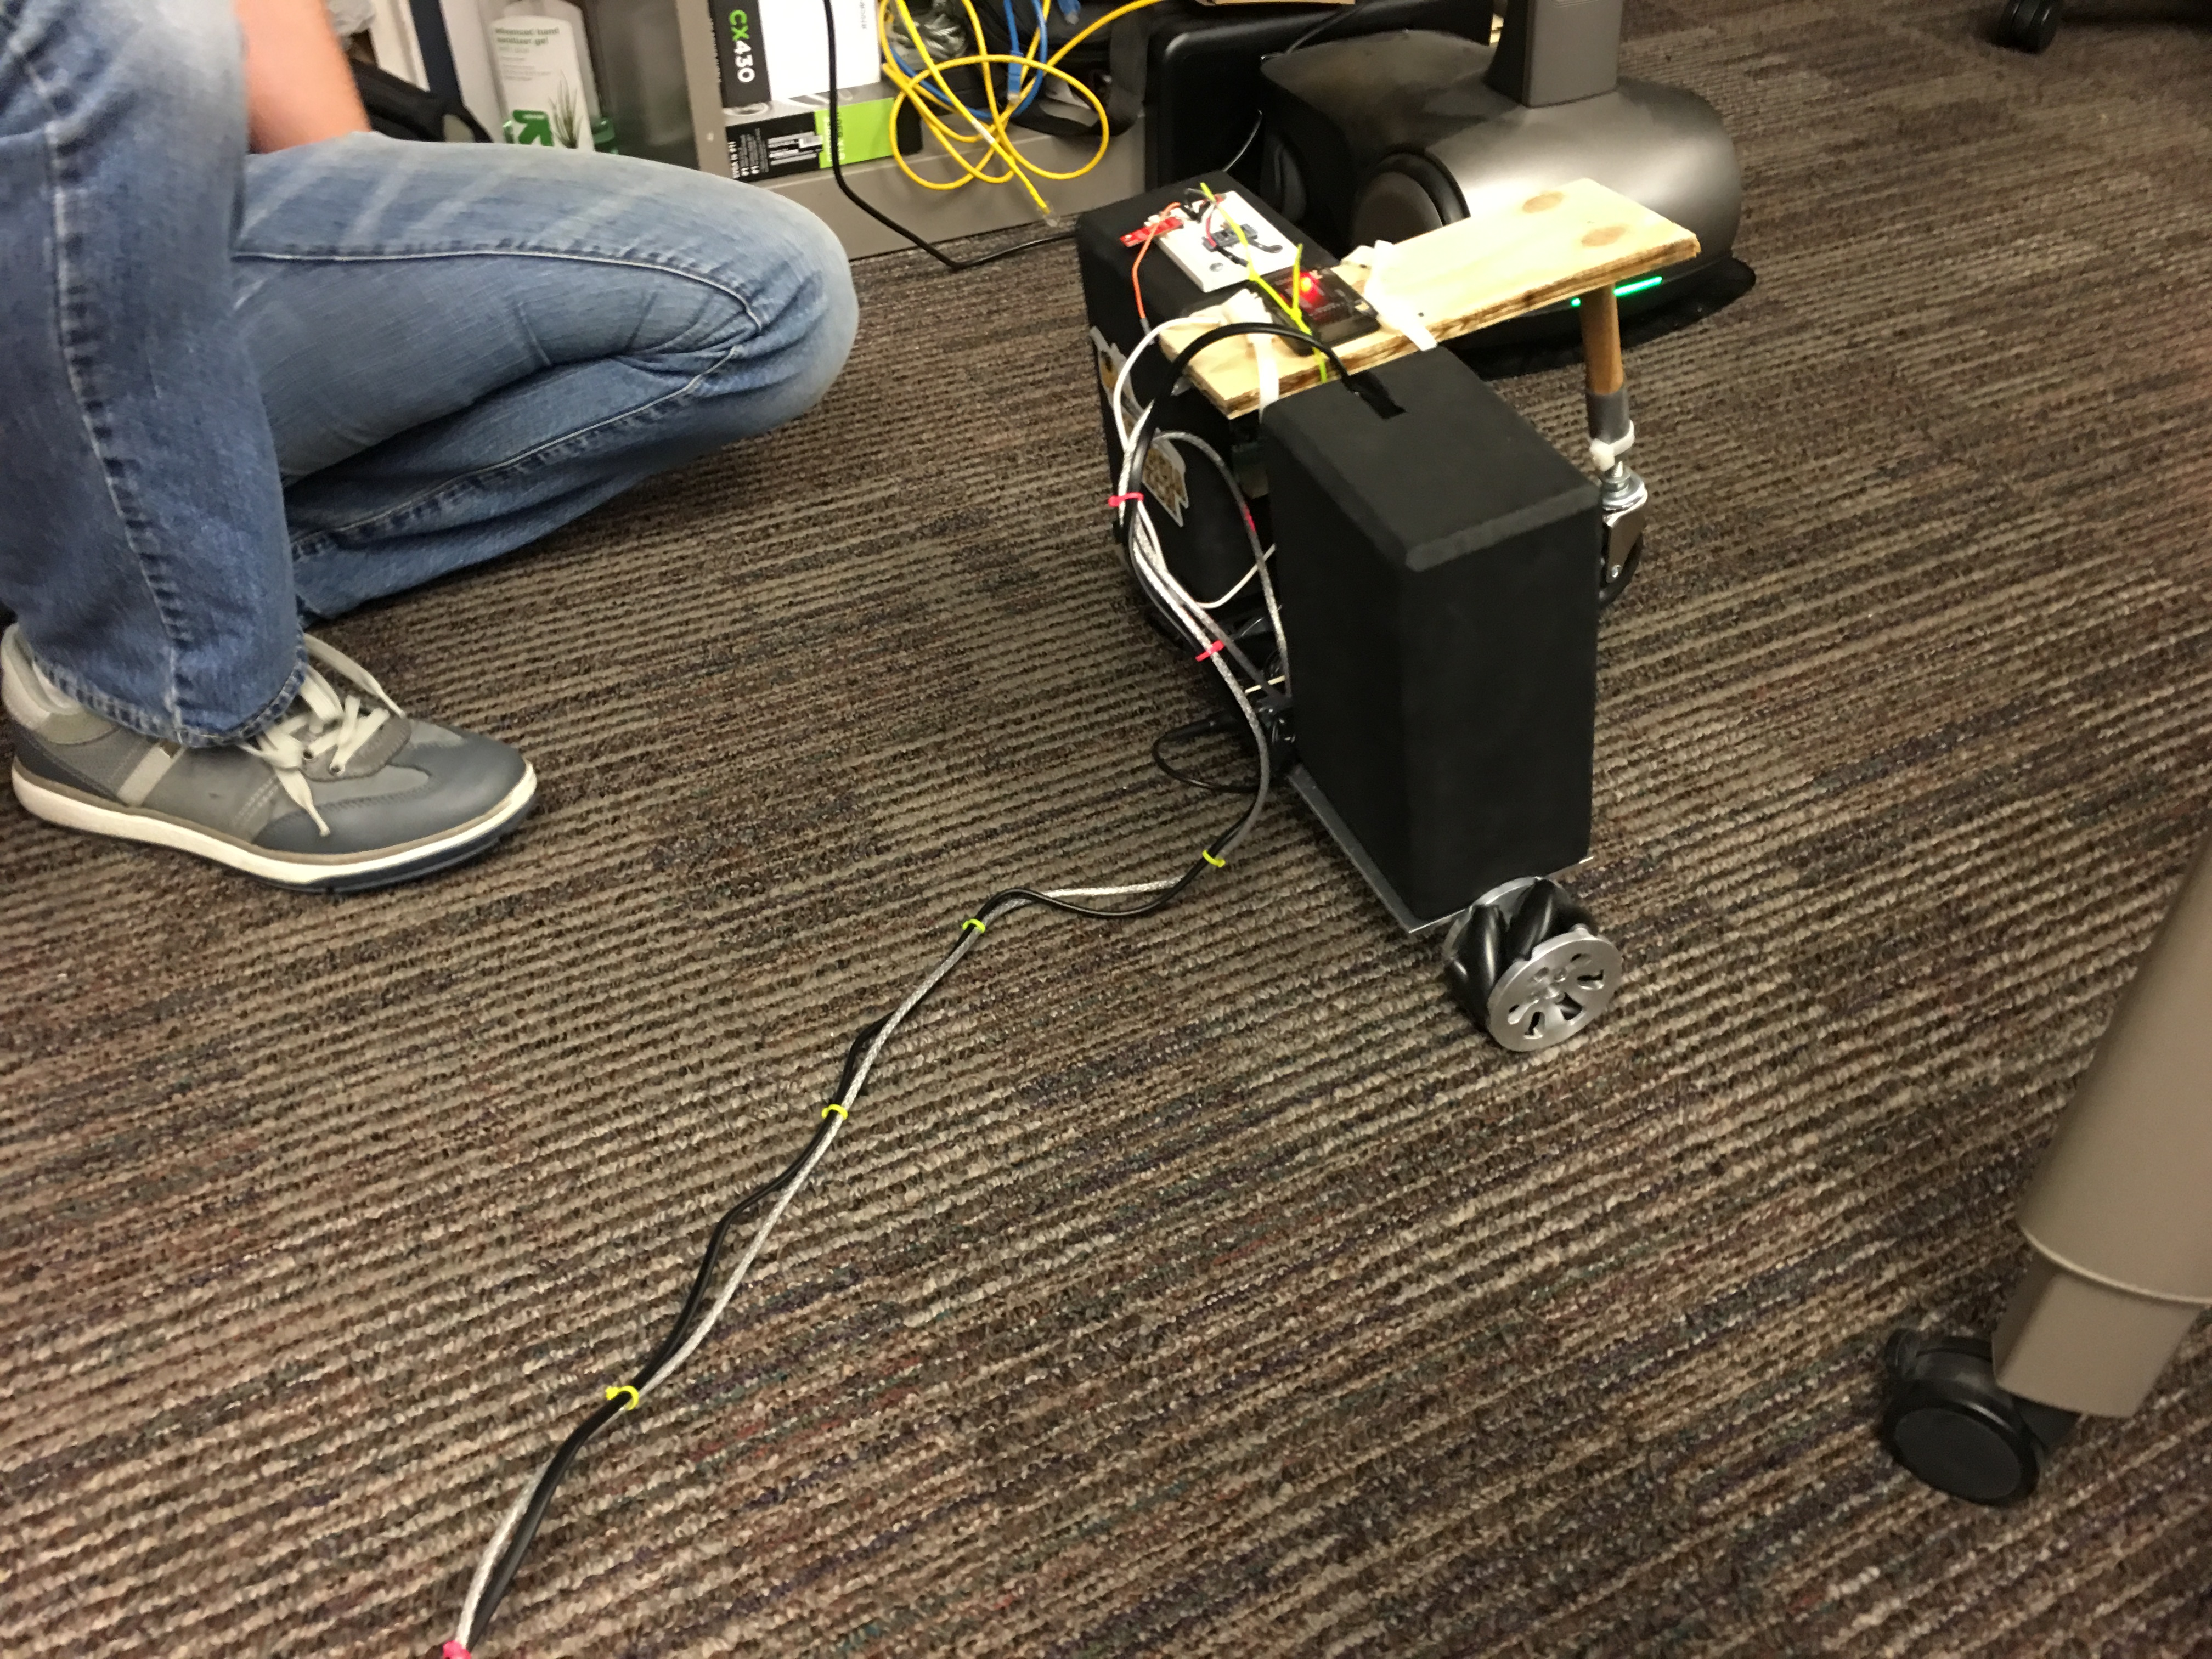
\includegraphics[width=\textwidth]{2016-05-05_04_21_25.jpg}
  \caption{The Balancing Golem Wing}
  \label{fig:balancing}
\end{figure}
In the end our software and hardware stack managed to balance the robot albeit with some oscillation caused by the controller. Although we tried a wide range of parameters for our PID controller, the robot continued to oscillate even in the most stable configurations. We can attribute this to the exceedingly low center of mass of the robot. Even with a fast control loop the wheels are unable to keep it stable without oscillation.\par
We also performed stress tests on this control loop. Under some configurations we managed to obtain good recovery after perturbation of the system but it didn't always recover. The Golem Wing remains fairly unstable by design and thus an interesting control problem.\par

\begin{figure}
  \centering
  \begin{subfigure}{0.3\textwidth}
    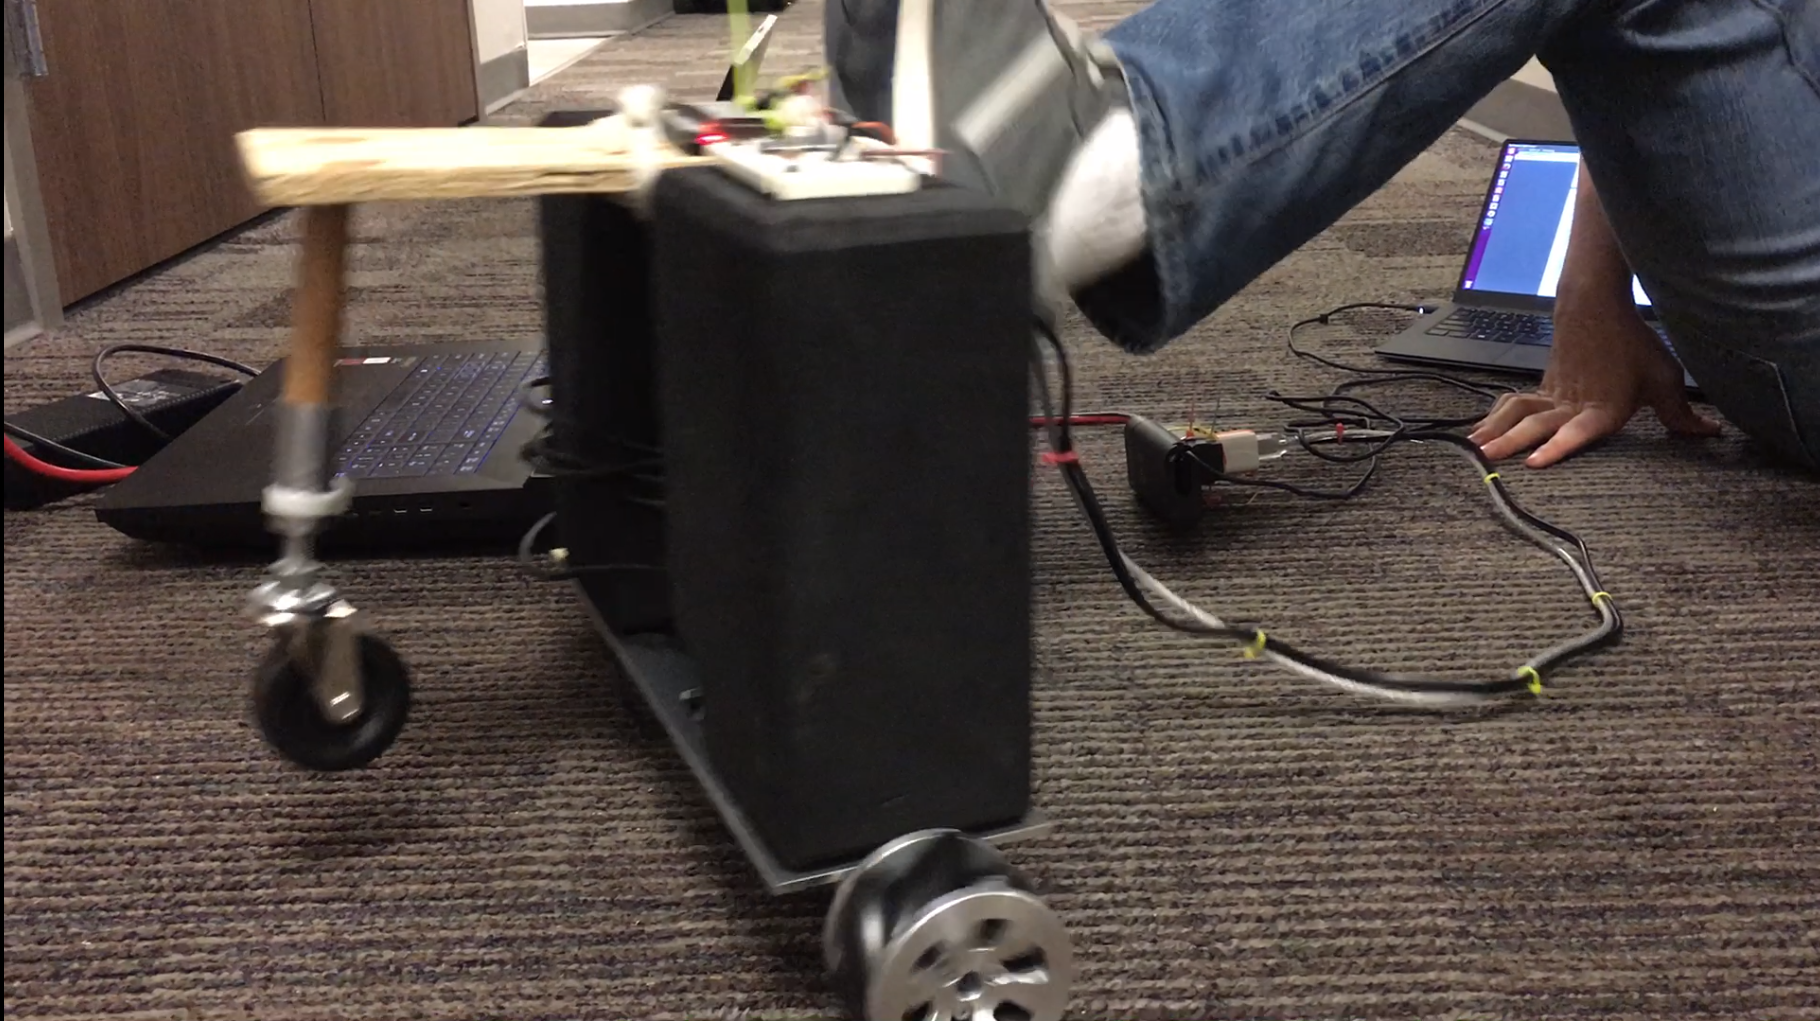
\includegraphics[width=\textwidth]{getting_kicked.png}
  \end{subfigure}
  \begin{subfigure}{0.3\textwidth}
        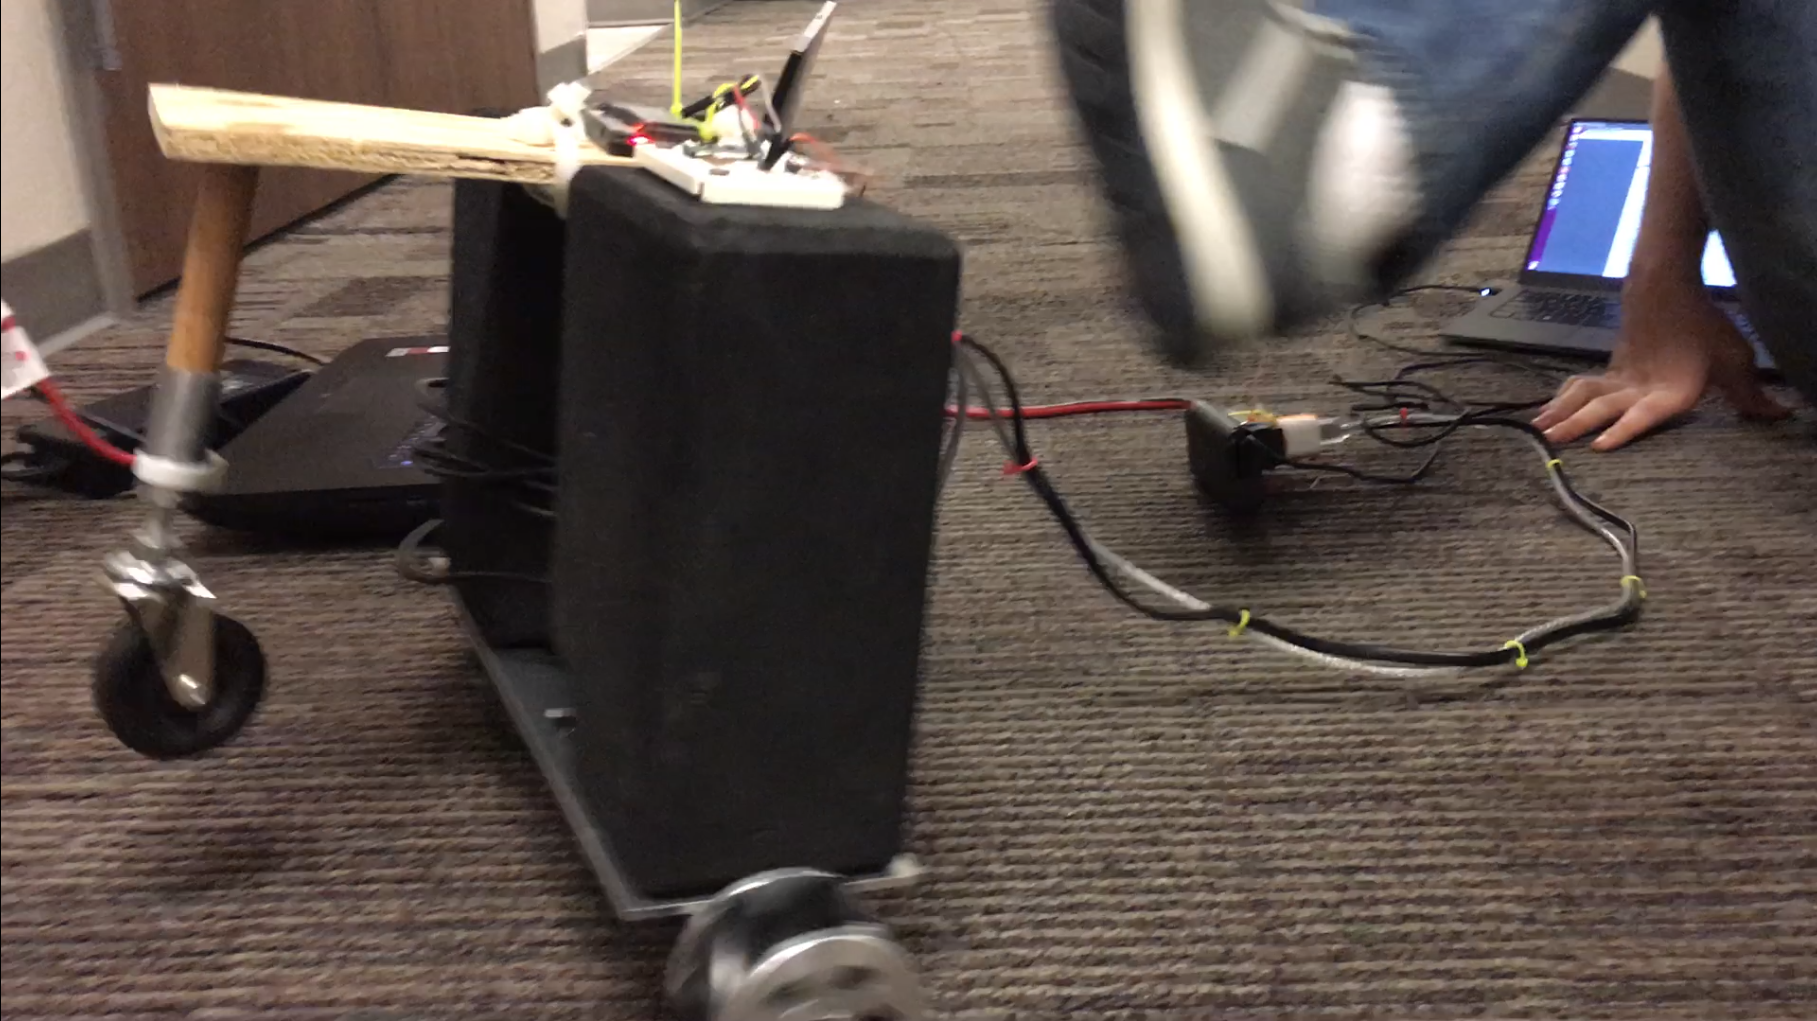
\includegraphics[width=\textwidth]{recovery.png}
  \end{subfigure}
  \begin{subfigure}{0.3\textwidth}
        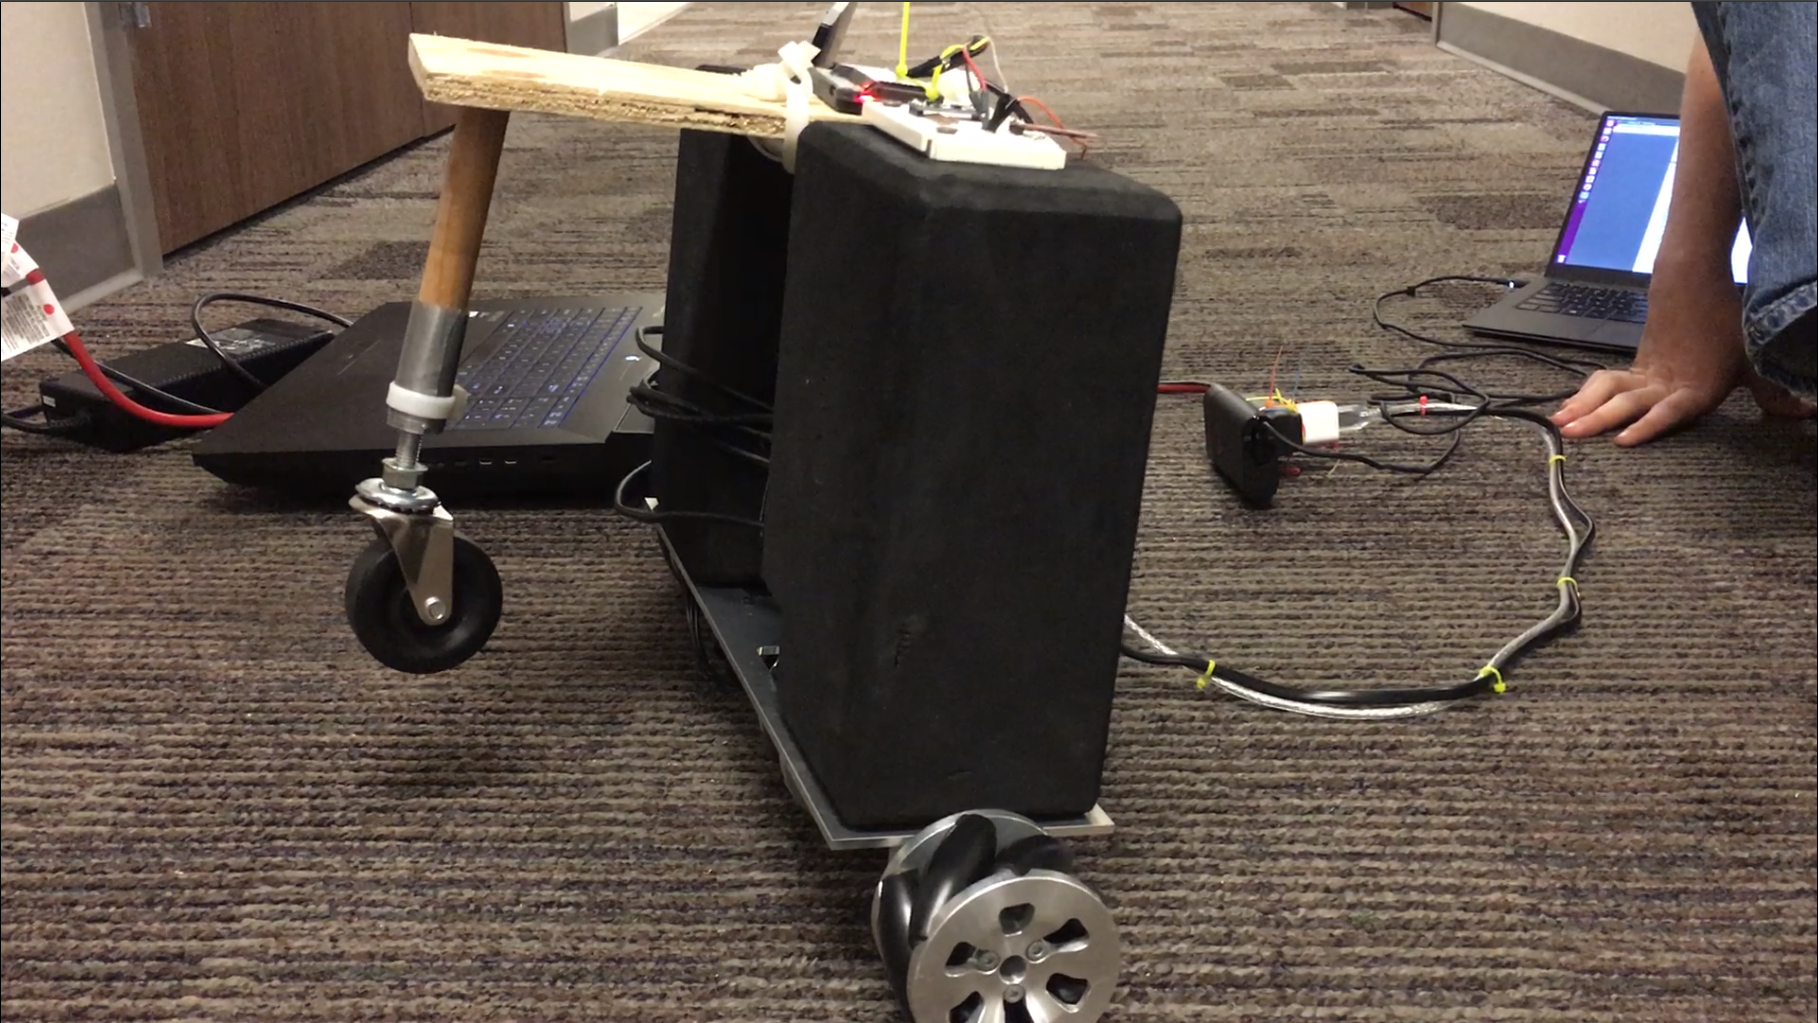
\includegraphics[width=\textwidth]{recovered.png}
  \end{subfigure} 
  \caption{Perturbation and recovery}
  \label{fig:pertandrec}
\end{figure}
 


\pagebreak
\printbibliography{}
\end{document}

